\documentclass{beamer}
\usepackage[utf8]{inputenc}

\usetheme{Madrid}
\usecolortheme{default}
\usepackage{amsmath,amssymb,amsfonts,amsthm}
\usepackage{txfonts}
\usepackage{multicol}
\usepackage{tkz-euclide}
\usepackage{listings}
\usepackage{adjustbox}
\usepackage{array}
\usepackage{tabularx}
\usepackage{gvv}
\usepackage{lmodern}
\usepackage{circuitikz}
\usepackage{tikz}
\usepackage{graphicx}
\usepackage{hyperref}
\usepackage{siunitx}

\setbeamertemplate{page number in head/foot}[totalframenumber]

\usepackage{tcolorbox}
\tcbuselibrary{minted,breakable,xparse,skins}



\definecolor{bg}{gray}{0.95}
\DeclareTCBListing{mintedbox}{O{}m!O{}}{%
  breakable=true,
  listing engine=minted,
  listing only,
  minted language=#2,
  minted style=default,
  minted options={%
    linenos,
    gobble=0,
    breaklines=true,
    breakafter=,,
    fontsize=\small,
    numbersep=8pt,
    #1},
  boxsep=0pt,
  left skip=0pt,
  right skip=0pt,
  left=25pt,
  right=0pt,
  top=3pt,
  bottom=3pt,
  arc=5pt,
  leftrule=0pt,
  rightrule=0pt,
  bottomrule=2pt,
  toprule=2pt,
  colback=bg,
  colframe=orange!70,
  enhanced,
  overlay={%
    \begin{tcbclipinterior}
    \fill[orange!20!white] (frame.south west) rectangle ([xshift=20pt]frame.north west);
    \end{tcbclipinterior}},
  #3,
}
\lstset{
    language=C,
    basicstyle=\ttfamily\small,
    keywordstyle=\color{blue},
    stringstyle=\color{orange},
    commentstyle=\color{green!60!black},
    numbers=left,
    numberstyle=\tiny\color{gray},
    breaklines=true,
    showstringspaces=false,
}
%------------------------------------------------------------
%This block of code defines the information to appear in the
%Title page
\title %optional
{10.7.53}
\date{October 4,2025}
%\subtitle{A short story}

\author % (optional)
{Aditya Appana - EE25BTECH11004}

\begin{document}


\frame{\titlepage}
\begin{frame}{Question}
Let $C_1$ and $C_2$ be respectively, the parabolas $x^2 = y- 1$ and $y^2 = x - 1$. Let $\vec{P}$ be any
point on $C_1$ and $\vec{Q}$ be any point on $C_2$. Let $\vec{P}_i$ and $\vec{Q}_i$ be the reflections of $\vec{P}$ and $\vec{Q}$
respectively with respect to the line $y = x$. Prove that $\vec{P}_i$ lies on $C_2$, $\vec{Q}_1$ lies on $C_1$,
and $\vec{P}\vec{Q} \geq min(\vec{PP_1}, \vec{QQ_1})$. Hence or otherwise determine points $\vec{P}_0$ and $\vec{Q}_0$  on the parabolas $C_1$ and $C_2$ respectively such that $\vec{P}_0\vec{Q}_0 \leq \vec{PQ}$ for all pairs of points $(\vec{P}, \vec{Q})$
with $\vec{P}$ on $C_1$ and $\vec{Q}$ on $C_2$.
\end{frame}



\begin{frame}[fragile]
    \frametitle{Solution}
The representation of a conic in vector form is \begin{align}\vec{x^T}\vec{V}\vec{x} + 2\vec{u^T}\vec{x}+f = 0\end{align}\\
$x^2 = y- 1$ represented in this form is:
\begin{align}\vec{x^T}\myvec{1&0\\0&0}\vec{x} + 2\myvec{0 \\ -\frac{1}{2}}^T\vec{x}+1 = 0\end{align}\\
$y^2 = x- 1$ represented in this form is:
\begin{align}\vec{x^T}\myvec{0&0\\0&1}\vec{x} + 2\myvec{-\frac{1}{2}\\0}^T\vec{x}+1 = 0\end{align}\\
\end{frame}


\begin{frame}[fragile]
    \frametitle{Solution}
Given $\vec{P}$ lies on (1), and given $\vec{P_i}$ is the mirror image of $\vec{P}$ with respect to line $y=x$. The mirror image $\vec{P_i}$ can therefore be represented as:
\begin{align} \vec{P_i} = \myvec{0&1\\1&0}\vec{P} \end{align}\\
If we want to prove that $\vec{P_i}$ lies on $C_2$, we need to show that $\vec{P_i}$ satisfies $C_2$.
\begin{align}
\brak{\myvec{0&1\\1&0}\vec{P}}^T\myvec{0&0\\0&1}\myvec{0&1\\1&0}\vec{P} + 2\myvec{-\frac{1}{2}\\0}^T\myvec{0&1\\1&0}\vec{P}+1 = 0\\
\vec{P}^T\myvec{0&1\\1&0}\myvec{0&0\\0&1}\myvec{0&1\\1&0}\vec{P} + 2\myvec{-\frac{1}{2}&0}\myvec{0&1\\1&0}\vec{P}+1 = 0
\end{align}\\
\end{frame}

\begin{frame}[fragile]
    \frametitle{Solution}
\begin{align}
\vec{P}^T\myvec{1&0\\0&0}\vec{P} + 2\myvec{0\\-\frac{1}{2}}^T\vec{P}+1 = 0
\end{align}
(7) is the same as $C_1$, so $\vec{P_i}$ satisfies $C_2$. In a similar manner, it can be proved that $\vec{Q_i}$ lies on $C_1$.\vspace{1cm}\\
\end{frame}


\begin{frame}[fragile]
    \frametitle{Solution and Plot}
We now need to prove $\vec{P}\vec{Q} \geq min(\vec{PP_1}, \vec{QQ_1}).$ Take $\vec{P}(1,2)$ and $\vec{Q}(5,2)$.
\begin{figure}[H]
    \centering
    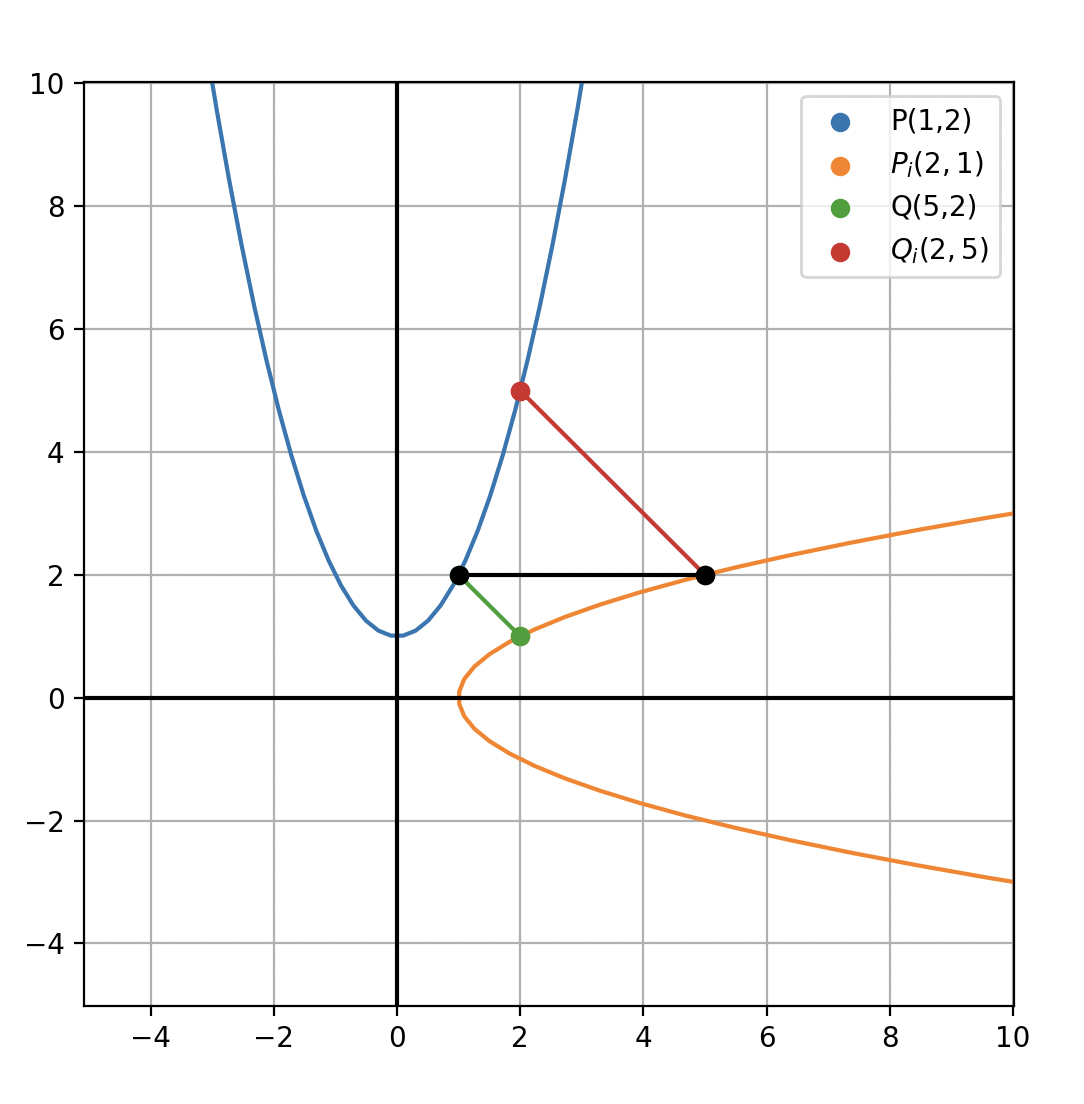
\includegraphics[width=0.5\columnwidth]{Figs/10753.png}
    \caption{Plot}
    \label{fig:placeholder}
\end{figure}
\end{frame}



\begin{frame}[fragile]
    \frametitle{Solution}
\begin{align} min(\vec{PP_1}, \vec{QQ_1}) = \vec{PP_i}\\
\norm{\vec{PP_i}} = \norm{\vec{P} - \vec{P_i} }= \norm{\myvec{1&0\\0&1}\vec{P} - \myvec{0&1\\1&0}\vec{P}} =
\sqrt{2}\norm{\myvec{\frac{1}{\sqrt{2}} &-\frac{1}{\sqrt{2}} \\ -\frac{1}{\sqrt{2}} & \frac{1}{\sqrt{2}}}\vec{P}}
\end{align}
Since the matrix is orthogonal, this equals:
\begin{align}
\sqrt{2}\norm{\vec{P}} = \sqrt{2}\times \sqrt{1^2 + 2^2} = \sqrt{10}
\end{align}
Now, $\norm{\vec{PQ}}$ = 
\begin{align}
    \sqrt{(5-1)^2 + (2-2)^2} = 4\\
\therefore \vec{PQ} \geq \vec{PP_i}\end{align}
\end{frame}

\begin{frame}[fragile]
    \frametitle{Solution}
We now need to find $\vec{P}_0$ and $\vec{Q}_0$ on the parabolas $C_1$ and $C_2$ respectively such that $\vec{P}_0\vec{Q}_0 \leq \vec{PQ}$ for all pairs of points $(\vec{P}, \vec{Q})$
with $\vec{P}$ on $C_1$ and $\vec{Q}$ on $C_2$. \vspace{1cm}\\
The line of shortest distance will be normal to both parabolas, and it will be perpendicular to the line $y=x$. Therefore the tangents at the point of intersection of line of shortest distance and the parabola will have same slope as $y=x$, $m=1$.\vspace{1cm}\\
The equation of tangent to a conic in vector form can be expressed as:
\begin{align}
    \vec{m}^T(\vec{Vq} + \vec{u}) =0
\end{align}
\end{frame}

\begin{frame}[fragile]
    \frametitle{Solution}
Where $\vec{m}$ is slope of tangent, and $\vec{q} = \myvec{x\\y}$ is the point of contact.
Substituting the values from (2), we get:
\begin{align}
    \myvec{1\\1}^T\brak{\myvec{1&0\\0&0}\vec{q} + \myvec{0\\-\frac{1}{2}}} = 0\\
    \myvec{1&1}\myvec{1&0\\0&0}\vec{q} + \myvec{1 & 1}\myvec{0\\-\frac{1}{2}} = 0\\
    \myvec{1&0}\myvec{x\\y} -\frac{1}{2} = 0\\
    x - \frac{1}{2} = 0\\
    x = \frac{1}{2}
\end{align}

\end{frame}
\begin{frame}[fragile]
    \frametitle{Solution}
Substituting the value of $x$ in (2), we get $y = \frac{5}{4}$. Therefore:
\begin{align}
\vec{P_0} = \myvec{\frac{1}{2} \\ \frac{5}{4}}\\
\vec{Q_0} = \myvec{0&1\\1&0}\vec{P_0} = \myvec{\frac{5}{4} \\ \frac{1}{2}}
\end{align}
\end{frame}


\begin{frame}[fragile]
    \frametitle{Codes}
\href{https://github.com/AdityaAppana/ee1030-2025/tree/c75597a082af90e6a6b10c85ca79d06aa3d9b661/ee25btech11004/matgeo/10.7.53/Codes}{Codes Permalink}
\end{frame}

\end{document}